\section{Example}
\label{sec:example}

To illustrate major steps of our approach, we use JLCA (a Java-to-C\# translation tool) as an example translation tool, and the \CodeIn{java. io.ByteArrayInputStream} class in Java as an example API element. TeMAPI includes three major steps to detect behavioral differences that are related to the example class from the mapping relations defined in the example tool.

%----------------------------------------------------
\textbf{Translating Synthesized wrappers.} TeMAPI first synthesizes the \CodeIn{Test\_java\_io\_ByteArrayInputStream} Java wrapper class for the example class. After that, we use JLCA to translate the wrapper class to C\#. TeMAPI compares source code of the synthesized wrapper class with source code of the translated one for translatable API elements of the example class. In particular, as described by its documentation\footnote{\url{http://tinyurl.com/2dsgftv}}, the example class in Java has five fields, two constructors, and eight methods besides inherited ones. A class can have more than one constructor, and a translation tool may not translate all its constructors. To extract API elements at the finest level, TeMAPI takes constructors into consideration when it synthesizes a wrapper method for each field/method of the example class. For example, given the \CodeIn{ByteArrayInputStream(byte[])} constructor, TeMAPI synthesizes the wrapper method as follows for the \CodeIn{skip(long)} method:

\begin{CodeOut}\vspace*{-1ex}
\begin{alltt}
public long testskip24nm(long m0, byte c0[])\{
  ByteArrayInputStream obj = new ByteArrayInputStream(c0);
  return obj.skip(m0);\}
\end{alltt}
\end{CodeOut}\vspace*{-2ex}

We next use JLCA to translate synthesized wrapper methods from Java to C\#. A translation tool typically cannot include mapping relations for all the API elements between two languages, so translated wrapper methods can have compilation errors. TeMAPI parses translated wrapper methods and removes all methods with compilation errors. For example, below is the translated \CodeIn{testskip- 24nm} method in C\#:
\vspace*{-2ex}

\begin{CodeOut}
\begin{alltt}
public virtual long testskip24nm(long m0, sbyte[] c0)\{
  MemoryStream obj = new MemoryStream(
                    SupportClass.ToByteArray(c0));
  MemoryStream temp_BufferedStream = obj;
  Int64 temp_Int64 = temp_BufferedStream.Position;
  temp_Int64 = temp_BufferedStream.Seek(m0,
       System.IO.SeekOrigin.Current) - temp_Int64;
  return temp_Int64;\}
\end{alltt}
\end{CodeOut}\vspace*{-2ex}

TeMAPI does not remove this method, since it does not result in compilation errors.


\textbf{Testing wrappers.} Besides, after translation, all translated code is within the wrapper method, and the names and parameter orders of a wrapper method are not changed. By checking whether a synthesized wrapper method returns the same value with its translated one given the same inputs, TeMAPI further tests wrapper methods for behavioral differences between mapped API elements. In particular, TeMAPI extends Pex~\cite{tillmann2008pex} to generate test cases for each remaining C\# wrapper method. For the example class, each wrapper method exposes all the inputs and output of a method and a constructor. As a result, Pex can change its inputs to exercise all feasible paths of its wrapped constructors and methods. Based on the inputs and output for each path, TeMAPI generate a Java test case to ensure that synthesized wrapper methods return the same values with translated ones. For example, TeMAPI generates the following Java test case based on inputs generated by Pex for one feasible path (in the C\# wrapper method) that throws exceptions.

\begin{CodeOut}\vspace*{-1ex}
\begin{alltt}
public void testskip24nm36()\{
  try\{
     Test_java_io_ByteArrayInputStream obj =
        new Test_java_io_ByteArrayInputStream();
     long m0 = java.lang.Long.valueOf(
                  "2147483648").longValue();
     byte[] c0 = new byte[0];
     obj.testskip24nm(m0,c0);
  \}catch(java.lang.Exception e)\{
     Assert.assertTrue(true);return;
  \}
  Assert.assertTrue(false);\}
\end{alltt}
\end{CodeOut}\vspace*{-2ex}

This Java test case fails, since given the preceding inputs, the \CodeIn{skip (long)} method in Java does not throw any exceptions as the translated C\# code does. Thus, TeMAPI detects a behavioral difference between the \CodeIn{skip(long)} method in Java and its translated C\# API elements by JLCA.

%-----------------------------------
\textbf{Testing sequences.} Pex is limited in generating sequences as pointed out by Thummalapenta \emph{et al.}~\cite{thummalapenta09:mseqgen}, so TeMAPI extends Randoop~\cite{pacheco2007feedback} for testing Java code to generate invocation sequences. TeMAPI does not choose to generate invocation sequences from wrappers directly since each wrapper method contain a fixed simple invocation sequence. Instead, by comparing the source code of synthesized wrapper methods with the source code of translated wrapper methods without compilation errors, TeMAPI first extracts all the translatable API methods of JLCA. When generating invocation sequences, TeMAPI limits its search scope, so that generated test cases invoke only translatable API methods. For example, a generated Java test case is as follows:

\begin{CodeOut}\vspace*{-1ex}
\begin{alltt}
public void test413() throws Throwable\{
  ...
  ByteArrayInputStream var2=new ByteArrayInputStream(...);
  var2.close();
  int var5=var2.available();
  assertTrue(var5 == 1);\}
\end{alltt}
\end{CodeOut}\vspace*{-2ex}


The test case gets passed since Java allows programmers to access the stream even if the stream is closed. We next use JLCA to translate the generated Java test case from Java to C\#. As the Java test case uses only translatable API elements, JLCA translates it to a C\# test case as follows:

\begin{CodeOut}\vspace*{-1ex}
\begin{alltt}
public void test413() throws Throwable\{
  ...
  MemoryStream var2 = new MemoryStream(...);
  var2.close();
  long available = var2.Length - var2.Position;
  int var5 = (int) available;
  AssertTrue(var5 == 1);\}
\end{alltt}
\end{CodeOut}\vspace*{-2ex}

If the translated test case has the same behaviors with the test case generated by Randoop, it should also get passed. However, the C\# test case gets failed since C\# does not allow such accesses and it throws \CodeIn{ObjectDisposedException}. TeMAPI thus detects a behavioral difference with invocation sequences.

This example motivates our basic idea of generating test cases in one language and translating those test cases to another language for detecting differences among API mapping relations. %We next present details of our approach.

%\begin{figure}[t]
%\centering %\hfill
%\includegraphics[scale=0.95,clip]{figure/sample.eps}\vspace*{-3ex}
% \caption{\label{fig:example}API mapping}\vspace*{-4ex}
%\end{figure}

%Based on the mapping relations, a translation tool can migrate the
%preceding code snippet automatically. To learn the mapping
%relations,
%
%%\begin{figure}[t]
%%\centering
%%\includegraphics[scale=0.86,clip]{figure/openfile.eps}\vspace*{-1.5ex}
%% \caption
%%{\label{fig:openfile}Aligned wrapper}\vspace*{-2ex}
%%\end{figure}
%
%In this section, we illustrate the main steps of MAM to
%mine the API mapping in Java for \CodeIn{System.IO.Directory.
%Exists()} in C\# from the HypoLog
%project\footnote{\url{http://sourceforge.net/projects/twlog/}}.
%
%The first step of MAM is to align classes and methods of
%wrapper by names. This step finds class pairs and method pairs
%that implement similar functionalities, and each pair may use
%API mapping since it implements a similar functionality. Our
%approach chooses names to align classes and methods because these
%classes and methods are from the same project. In this example, our
%approach aligns the two methods as shown in
%Figure~\ref{fig:openfile} because the two method have similar names
%and their declaring classes also have similar names (see
%Section~\ref{sec:approach:alignclientcode} for details).
%
%The second step of MAM is to mine mapping relations of API
%classes based on the names of corresponding fields, parameters,
%returned types, and local variables. This step also relies on names
%for the same consideration of the first step. For example, our
%approach maps the two parameters with the same name as shown by the
%red arrow of Figure~\ref{fig:openfile}. From the types of the two
%parameters, MAM mines the mapping relation between two API
%classes: \CodeIn{System.String} $\leftrightarrow$
%\CodeIn{java.lang.String} (see
%Section~\ref{sec:approach:mappingtypes} for details).
%
%
%The final step of MAM is to mine mapping relations of API
%methods. Besides the factors listed in
%Section~\ref{sec:introduction}, another factor is that API calls in
%wrapper are often not carefully aligned. To deal with those
%challenges, MAM first builds an API Transformation Graph
%(ATG) for each method. After that, MAM compares built
%graphs to mine mapping relations of API methods (see
%Section~\ref{sec:approach:mappingtypes} and
%Figure~\ref{fig:approach1} for details). Figure~\ref{fig:example}
%shows the mined mapping relation between
%\CodeIn{System.IO.Directory.Exists()} and its API mapping in
%Java.
